% !TeX spellcheck = en_US
\documentclass[a4paper,12pt]{article}
\usepackage{listings}
%\usepackage[T1]{fontenc}
\usepackage{fontspec}
\usepackage[greek, english]{babel}
\usepackage[super]{nth}
\usepackage{fancyhdr}
\usepackage[left=1.50cm, right=1.50cm, top=2cm, bottom=1.cm, includeheadfoot]{geometry}
\usepackage{amsmath}
\usepackage{graphicx}
\usepackage{subcaption}
\usepackage{float}
%\usepackage[colorinlistoftodos]{todonotes}
\usepackage{xcolor}
\usepackage{ulem}
\usepackage{amsmath}
\usepackage{caption}
\usepackage{subcaption}
\usepackage{tabularray}
\usepackage[framed]{matlab-prettifier}
\usepackage{svg}
\usepackage{nth}
\usepackage{wrapfig}
\usepackage{siunitx}
\usepackage{bm}
\usepackage{algorithm}
\usepackage{algpseudocode}
\usepackage{dirtytalk}
\usepackage{gensymb}
\usepackage{enumerate}

\usepackage[pdfauthor={Alexandra Gianni, Nikos Stylianou},
pdftitle={Second Problem Set},
pdfcreator={TeX},
pdfsubject={ECE447 - Neuro-Fuzzy Computing}]{hyperref}


\sisetup{output-exponent-marker=\ensuremath{\mathrm{e}}}

\hypersetup{
	colorlinks,
	citecolor=blue,
	filecolor=black,
	linkcolor=black,
	urlcolor=blue
}

\lstset{
	style              = Matlab-editor,
	basicstyle         = \footnotesize,
	escapechar         = ",
	mlshowsectionrules = true,
}

%\setmainfont{Times New Roman}
\setmainfont{TeX Gyre Termes}

\pagestyle{fancy}
\fancyhf{}
\fancyhead[l]{\footnotesize \nth{3} Problem Set}
\fancyhead[r]{\footnotesize Neuro-Fuzzy Computing}
%\fancyfoot[r]{\footnotesize \thepage}
\renewcommand{\footrulewidth}{0.4pt} % Line at the footer visible

\fancyfoot[c]{\thepage}

\fancypagestyle{first}{
	\fancyhf{}
	\renewcommand{\headrulewidth}{0pt}
	\fancyfoot[c]{{\large \today}}
	\renewcommand{\footrulewidth}{0.0pt} % Line at the footer visible
} 

\newcommand{\MathSpace}{\ }
\setlength{\parindent}{0pt} % Paragraph identation is set to 0

\newcommand\ddfrac[2]{\frac{\displaystyle #1}{\displaystyle #2}} % Better fractions for inline

\renewcommand{\thesubsection}{(\alph{subsection})} % Change subsection style
\renewcommand{\thesection}{\hspace{-18pt}} % Make section style look nicer
\renewcommand\thesubsubsection{\thesection\hspace{18pt}(\alph{subsection}). \roman{subsubsection}}

\definecolor{veraman}{HTML}{55928A}

\begin{document}
	
	\begin{titlepage}
		\thispagestyle{first}
		
		\newcommand{\HRule}{\rule{\linewidth}{0.5mm}} % Defines a new command for the horizontal lines, change thickness here
		
		\center % Center everything on the page
		
		%----------------------------------------------------------------------------------------
		%	HEADING SECTIONS
		%----------------------------------------------------------------------------------------
		
		\textsc{\LARGE University of Thessaly}\\[1.6cm] % Name of your university/college
		
\includegraphics[scale=.5]{Images/uth-logo.png}\\[1cm] % Include a department/university logo - this will require the graphicx package
		\textsc{\Large Neuro-Fuzzy Computing}\\[0.6cm] % Major heading such as course name
		\textsc{\large ECE447}\\[0.5cm] % Minor heading such as course title
		
		%----------------------------------------------------------------------------------------
		%	TITLE SECTION
		%----------------------------------------------------------------------------------------
		
		\HRule \\[0.5cm]
		{ \huge \nth{3} Problem Set}\\[0.4cm] % Title of your document
		\HRule \\[1.8cm]
		
		%----------------------------------------------------------------------------------------
		%	AUTHOR SECTION
		%----------------------------------------------------------------------------------------
		
		
		\vspace*{1cm}
		\begin{minipage}{\textwidth}
			\centering
			\begin{tblr}{cc}
				\emph{{\LARGE Alexandra Gianni}} & \emph{{\LARGE Nikos Stylianou}} \\ [3mm]
				\emph{{\LARGE ID: 3382}} & \emph{{\LARGE ID: 2917}} \\
			\end{tblr}
		\end{minipage}\\[2.5cm]
		
		% If you don't want a supervisor, uncomment the two lines below and remove the section above
		%\Large \emph{Author:}\\
		%John \textsc{Smith}\\[3cm] % Your name
		
		%----------------------------------------------------------------------------------------
		%	DATE SECTION
		%----------------------------------------------------------------------------------------
		
		
		%\vfill % Fill the rest of the page with whitespace
		
	\end{titlepage}

	% !TeX spellcheck = en_US
\section{Problem 2}

We are asked to write a Python program that implements steepest descent algorithm for the 1-$S^1$-1 RBF network.
The input function that we want to approximate is 
\[
g(p) = 1 + \sin\left(p\pi/8\right), \quad \text{for} \ p \in \left[-4,4\right]
\]

We select 30 data randomly from that interval and all parameters are initialized as small numbers using \verb|numpy.random.randn| function. It returns a number at the exact specification as needed.

\begin{figure}[htbp]
	\centering
	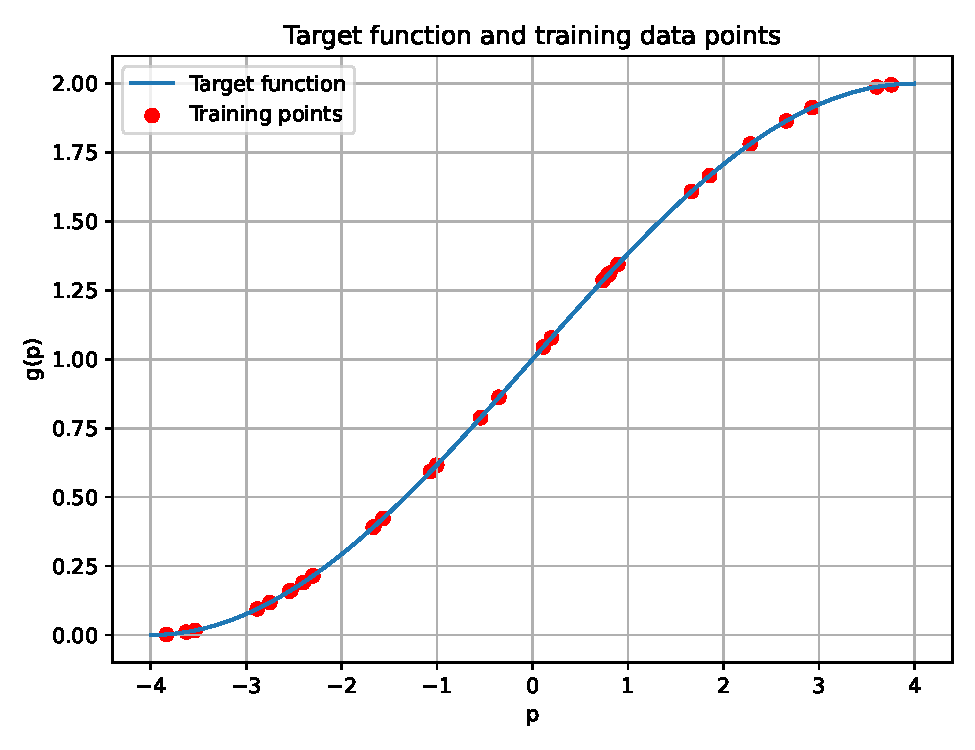
\includegraphics[width=0.6\linewidth]{../Problem 2/prob2_targetFunc_dataPoints.pdf}
	\caption{Input function in the specified area and the randomly assigned train data points.}
\end{figure}

For the randomly assigned data points, we added a custom seed number using in order for the results to be comparable but still use randomness.

	% !TeX spellcheck = en_US
\section{Problem 8}
The term "ordinary subset of level $\alpha$ in fuzzy set theory refers to a non-fuzzy subset that is created from a fuzzy subset by taking into consideration only those elements whose degrees of membership are at least $\alpha$. In essence, it's a threshold-based selection from a fuzzy set in which each element is only included if its membership score is greater than or equal to $\alpha$.\\
Conversely, this idea is extended to pairs of components for a fuzzy relation by the "ordinary relation of level $\alpha$". A set of ordered pairs with corresponding degrees of membership that indicate the strength of the relationship between the elements form a fuzzy relation. Thus, the set of all pairs whose membership in the fuzzy relation is at least $\alpha$ is the ordinary relation of level $\alpha$. \\

Analytically, the ordinary relation of level $\alpha$ for a fuzzy relation is defined as the set of all pairs $(x,y)$ for which the membership function $\mu_{\tilde{R}}(x,y)$ is greater than or equal to $\alpha$. Alternatively, it is a crisp set that is derived from the fuzzy relation by incorporating all element pairs with a degree of membership greater than the specified level $\alpha$\\

For a fuzzy relation with a membership function $\mu_{\tilde{R}}(x,y) = 1 - \frac{1}{1+x^2+y^2}$, the ordinary relation of level $0.3$ is the set:\\
\begin{equation}
	R_{0.3} = {(x,y) | \mu_{\tilde{R}}(x,y) \geq 0.3}
\end{equation}
This means you are looking for all the pairs $(x,y)$ where the membership value is at least $0.3$.\\

To determine analytically the ordinary relation of level $0.3$, we will solve the inequality
\begin{align*}
	\mu_{\tilde{R}}(x,y) \geq 0.3 \\
	1 - \frac{1}{1+x^2+y^2} \geq 0.3 \\
	\frac{1}{1+x^2+y^2} \leq 0.7 \\
	1 + x^2 + y^2 \geq \frac{1}{0.7} \\
	x^2 + y^2 \geq \frac{1}{0.7} - 1 \\
	x^2+y^2 \geq \frac{3}{7}
\end{align*}
From basic math we know that $	x^2 + y^2$ is the equation of a circle. This represents the region outside a circle centered at the origin with a radius of $\sqrt{\frac{3}{7}}$.This means the ordinary relation of level 
$0.3$ includes all $(x,y)$ pairs whose distance from the origin is at least 
$\sqrt{\frac{3}{7}}$.\\
To visualize this, we will plot a circle centered at the origin with a radius of 
$\sqrt{\frac{3}{7}}$.​
The area outside this circle represents the ordinary relation of level 
$0.3$.
\begin{figure}[H]
	\centering
	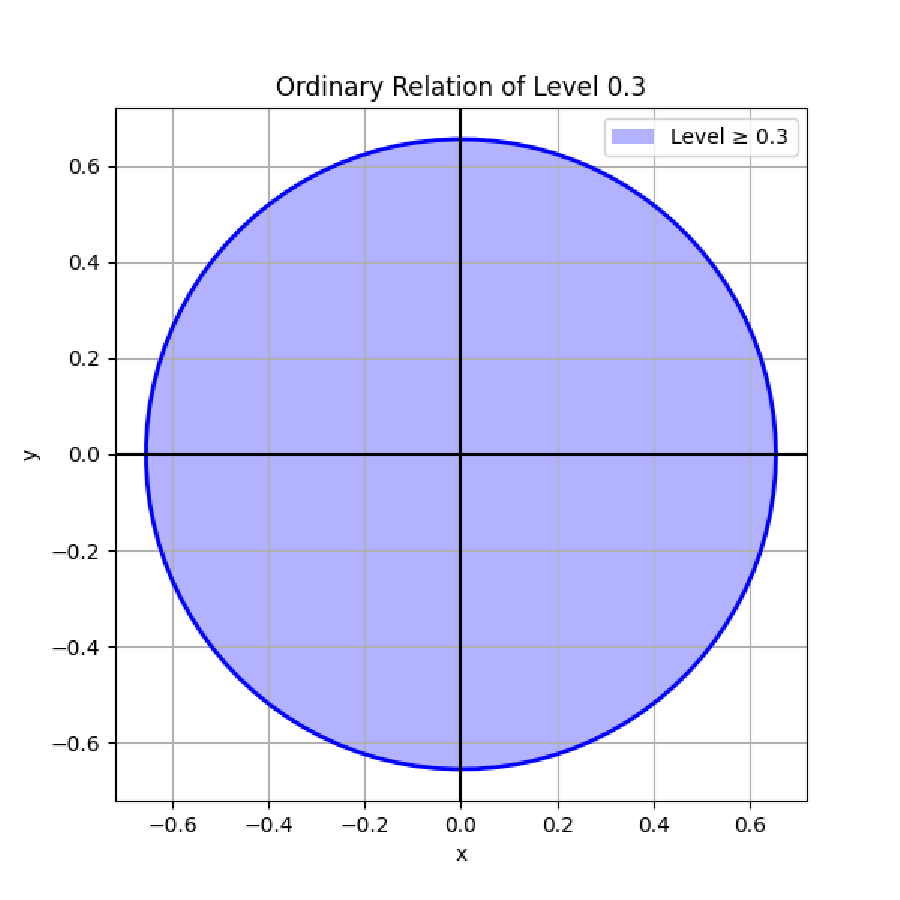
\includegraphics[width=0.5\textwidth]{../Problem 8/ordinary_plot.pdf}
	\caption{Ordinary relation of Level $0.3$}
\end{figure}
The plot above represents the ordinary relation of level $0.3$ for the given fuzzy relation. The blue shaded area, including the boundary, otside the circle indicates the region where the membership function is greater than or equal to 0.3. This area corresponds to all points $(x,y)$ whose distance from the origin is at least $\sqrt{\frac{3}{7}}$, as derived analytically. The boundary circle itself represents the exact threshold where the membership value $0.3$ and the area outside this circle encompasses all points with a membership value greater than $0.3$., fulfilling the condition for the ordinary relation of level 0.3. 
\\
The area enclosed by the circle is: Area = $1.346396851533$


	
	
\end{document}